\chapter{Development}

This chapter describes the development of my database application, SpiDB, from September 2015 to March 2016, involving planning, testing and implemention. The project is open-source, which can be found at
\textit{https://github.com/SpiNNakerManchester/SpiNNakerGraphFrontEnd}.

By being part of the SpiNNaker team in Manchester, I was directly exposed to the ongoing research, frequently receiving feedback on my work. The collaboration was effectively bi-directional, as I was able to constantly find, evaluate and fix inconsistencies and bugs in the API not known to the team.

\section{Planning and Design}
The project imposed a relatively steep learning curve, given the complexity of the low level distributed architecture, still under development. Given this, on the 5th? of September 2015, I attended the 5th? SpiNNaker workshop, where multiple researchers from around the globe gathered for a one week course on the basics of the hardware??. I was then officially introduced to the Manchester team... planning etc.

The plan involved splitting my project into two parts: building a NoSQL Key-value store and an SQL based Relational Database.

[blackboard is down...] get planning link

key-value then relational

\section{Implementation}

\subsection{Technologies Used}
The SpiNNaker API is split into the Python toolchain, running on the host machine (user's computer) and C code, compiled into machine code to run on the board. A strong knowledge of ARM assembly was also needed, given the low level architecture.
 
These technologies were used to develop the following deliverables:
\begin{itemize}
	\item \textbf{Python}: (2000 lines of code) uploading binaries to the board, status checking, query parsing, Graphical User Interface, data analytics and socket communication.
	\item \textbf{C}: (2500 lines of code) event driven communication between processors, low level memory management, distributed query processing.
\end{itemize}

\subsection{Approach}

A tree structure composed of \textit{root}, \textit{branch} and \textit{leaf} nodes. The tree structure presented by my database management system allows a divide and conquer approach to the database query plan. This means when queries are issued by the \textit{host}[definition] and received at the \textit{root}, they are broken down and forwarded for parallel processing through \textit{branch} and \textit{leaf} nodes. eg. COUNT, MAX, MIN, AVG, SUM

problems:
sending a large amount of packets with little or no delay xx kills xx the core. sending more than about 4 packets symultaneously at a destination results on a very high packet loss (2/3 of SDP packets get dropped).


solutions:...
delays
tree structure
no acknowledgement


This approach has the following advantages (compared to a flat structure)
-a core will only ever receive packets from up to 4 other cores symultaneously (branch: 4, root: 1, leaf: 1), which is the limit of reliability.
-aggregation of results can be done in iterations/stages

disadvantage:
-less leaf nodes (which do the actual work)

LIMITATION:
no global timer, the maximum we can do is a timer for each chip (collection of 18 cores)
reliability

COMPLEXITY

limitation:
-single point of failure for each board(mention that it is already like that. no way to avoid).
-SDRAM bandwidth

scalability

message id and all other fields, etc.

each chip, following instances:...

\begin{itemize}
\item 1x \textit{sark} - monitor process provided by the API to handle low level SpiNNaker operating system functions
\item 1x \textit{reinjector} - utility process provided by the API to allow automatic re-propagation of dropped multicast packets
\item 1x \textit{root} - central node which handles direct communication with host machine via UDP and redirects incomming queries to respective cores. 
\item 3x \textit{branch} - intermediate node which aggregates queries from 4 leaf nodes and communicates back to host via UDP (why 4? because 4 sdp channels?). 
\item 12x \textit{leaf} - receives insert/retrieve queries from the root, processes the request and then returns result to branch node
\end{itemize}
why branches, etc?

\begin{figure}
\begin{center}
	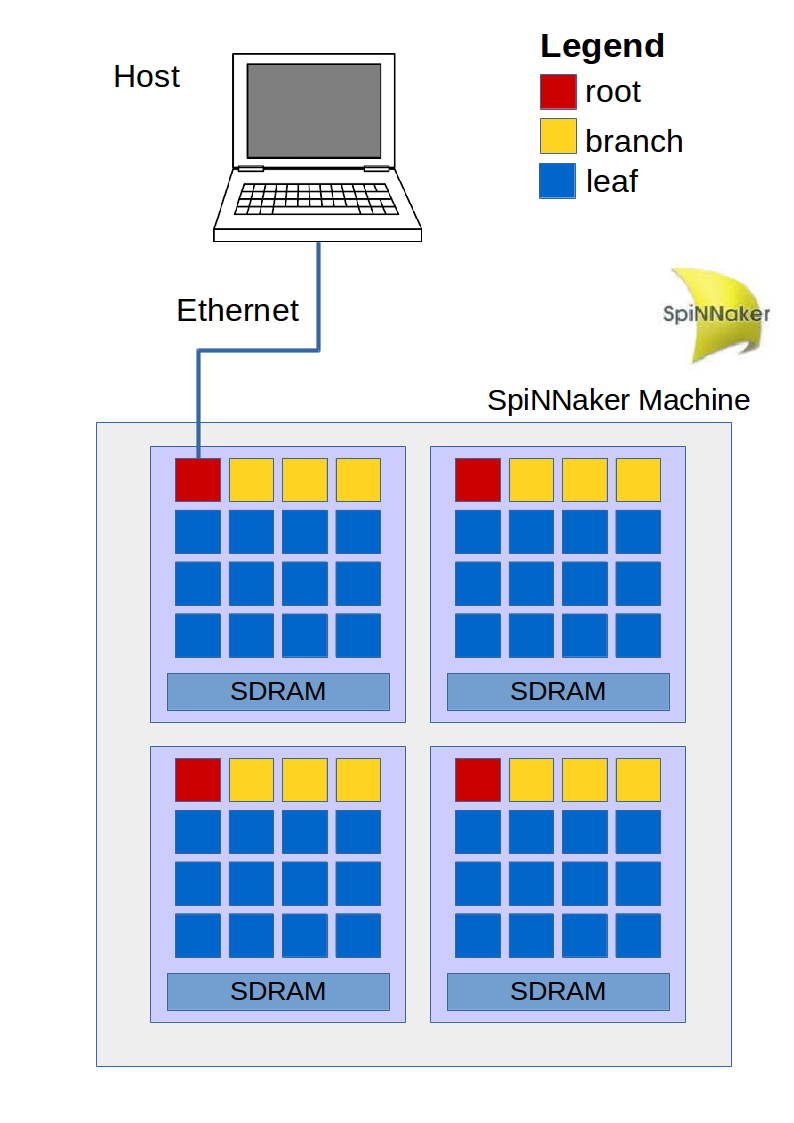
\includegraphics[width=0.8\textwidth, natwidth=794, natheight=1123]{images/spiDB_architecture.png}
\end{center}
\caption{SpiDB Architecture}
%\label{fig:die-plot}
\end{figure}

\subsection{Key-value Store}
\subsubsection{PUT}

DOT SYNTAX AND EXAMPLE CODE SQL KV.
graphs from ui and ui itself

Syntax:\\
\noindent
 {\large\textbf{put} \textit{(int|string)}:key \textit{(int|string)}:value} \\\\

The \textbf{put} operation is the main way of inserting data onto the SpiDB distributed database. 
Upon completion, such operation will store the specified key, mapping to its value, on the memory of an arbitrary chip in the Spinnaker board (as chosen by the root core). This operation expects an acknowledgement from the core which stored the entry.\\\\

\noindent
 Example usage:\\
 \begin{lstlisting}
 put "hello" "world"
 put 123 "foo"
 put "life" 42
 put 1 2
 \end{lstlisting}
\noindent 
 Complexity: linear to the size of the input key-value, constant to database size.\\\\
 
Steps:
\begin{enumerate}
\item User issues query of format \textit{put "key" "value"} on host machine
\item Query and metadata are converted into a byte array with the following format, transferred over UDP socket to the board

\lstinputlisting[language=C]{code/putQuery.c}

Where \textit{info} contains the metadata regarding the entry to be stored. It is composed of 32 bits, ...
[bits bits bits, etc]

how is it actually stored??? !!?!! say it and mention word alignment

\item Packet transfer triggers interrupt on \textit{root} core, which selects a \textit{leaf} core to store the data entry (hash or Round Robin...?) and communicates to it via SDP
\item \textit{leaf} triggers an interrupt and stores key-value entry into its dedicated region of SDRAM
\item \textit{leaf} sends an acknowledgement message over UDP back to host
\end{enumerate}

\subsubsection{PULL}


design decision: pull no reply....

 Syntax:
 \noindent
 {\large\textbf{pull} \textit{(int|string)}:key}\\\\
 
The \textbf{pull} operation is the main way of retrieving data from the SpiDB distributed database.
When the operation is issued, the SpiNNaker cores will be coordinated to search for the given key and, if found, the value mapped by it will be returned to host. If the key does not exist, no reply is given, resulting on a timeout on the host (reason for this...). This means 
-disadvantage: expensive if not found
-advantage: less packet drops as less internal communication traffic
 
\noindent
 Example usage:\\
 \begin{lstlisting}
 pull "hello"
 pull 123
 \end{lstlisting}
 Assuming successful execution of the put commands above, such pulls would return "world" and "foo" respectively.\\\\
 Complexity: linear to the size of the input, linear to database size.\\\\

\begin{enumerate}
\item User issues query of format \textit{pull "key"} on host machine
\item Query and metadata are converted into a byte array, transferred over UDP socket to board
\item Packet transfer triggers interrupt on \textit{root} core, which issues a \textit{multicast} packet to all \textit{leaf} nodes requesting them to search for occurences of "key"
\item \textit{leaf} triggers an interrupt
\begin{itemize}
\item If a \textit{leaf} node identifies "key" by scanning linearly through SDRAM, it responds to host (branch...?) with mapped value
\item Else no response is sent, yielding timeout on host (reason for this!!!...?)
\end{itemize}
\end{enumerate}


(benchmarking in chapter 3)
how the data is actually stored?

SQL:
column based?

bandwidth (max) vs throughput (actual)


identifies
flow control of:
put
pull
etc.

Upon completion of the project, 


\subsection{Relational Database}

\subsubsection{CREATE }
\noindent 
  {\large\textbf{CREATE TABLE} \textit{(string)}:tableName(\\
  	\textit{(string)}:column1 integer|varchar(\textit{int}),\\
  	\textit{(string)}:column2 integer|varchar(\textit{int}),\\
  	...\\
  	);}\\\\
\noindent
  Reserves memory space for an SQL table and stores its metadata. This operation expects an acknowledgement.\\\\
   Complexity: linear to the size of the input, constant to database size.\\\\
   
\subsubsection{INSERT}   
   
 \noindent
  {\large\textbf{INSERT INTO} \textit{(string)}:tableName(\textit{(string)}:column1,\textit{(string)}:column2,...)\\
  \textbf{VALUES}(\textit{(int|string)}:value1,\textit{(int|string)}:value2,...);}\\\\
\noindent
  Inserts specified values on the given table's memory space at an arbitrary chip. This operation expects an acknowledgement.\\\\
\noindent
   Complexity: linear to the size of the input, constant to database size.\\\\

\subsubsection{SELECT}   
   
\noindent
  {\large\textbf{SELECT} *|\textit{(string)}:column1,\textit{(string)}:column2,...\\
  \textbf{FROM} \textit{(string)}:tableName\\
  \textbf{WHERE} \textit{(string)}:column|\textit{(int|string)}literal \\=|!=|\textless |\textless =|
  \textgreater | \textgreater = \textit{(string)}:column|\textit{(int|string)}literal;}\\\\
\noindent
  Retrieves a list of entries corresponding to the previously inserted values on given table which match the WHERE criteria. Matching results are streamed in until timeout is reached. If no value matches the criteria, the Spinnaker board will not respond.\\\\
\noindent
Complexity: linear to the size of the input, linear to database size.\\\\
  
\subsection{Out-of-order execution}
As SpiNNaker is a distributed architecture, it may cause many issues and inconsistencies.
For example, if we try to execute the following code sequence in order:\\
\begin{lstlisting}[caption={Non-blocking execution}, label=list:non-blocking]
put "hello" "world"
pull "hello"
\end{lstlisting}

We are not guaranteed that the \textit{pull} query will retrieve the value "world". As both queries are executed symultaneously on the SpiNNaker board, there is a chance that the \textit{pull} operation will terminate before the \textit{put} does, thus failing to return a value.

As a solution to this dependency constraint, my SpiDB database API includes the syntax symbol "." (dot) which blocks execution until all preceeding operations terminate. This allows the programmer to control execution flow, choosing what is allowed to compute out-of-order (in parallel) and what should be sequentialised at a cost of performance. This is a similar concept to the Verilog blocking and non-blocking assignments.[?]

\begin{lstlisting}[caption={Blocking execution}, label=list:blocking1]
put "hello" "world"
.
pull "hello"
\end{lstlisting}

The above code will assure sequential code, meaning the \textit{pull} operation will always return "world". It is usually a good idea to block execution when given a dependency constraint. This can also be done with larger code fragments.

\begin{lstlisting}[caption={Blocking execution}, label=list:blocking2]
put "hello" "world"
put "life" 42
put 123 456
.
pull "hello"
pull "life"
pull 123
\end{lstlisting}

It is worth noting that although non-block operations can cause out-of-order execution, it does not occur very frequently. This is because, when transmitting data to the board, queries are serialised over ethernet in order of appearence and in addition there is a small forced transmission delay between these packets. This will be further discussed on chapter 3.%\autoref{cha:eval}.

\section{Testing and Debugging}
I started the project with a Test-Driven Development approach, writing Python tests with the \textit{unittest} module and C assertions with part of the SpiNNaker API module \textit{debug.h} and my own code. This allowed high reliability from the start.

Realtime debugging on the SpiNNaker board is relatively hard, but luckly the API provides ways to log messages in each core's private data memory, which can be read by an external process upon execution of the program. Debugging was performed with a tool named \textit{ybug}, also developed by the team, which allows core status checking, uploading binaries, reading logs and memory content, among other functionality.\cite{ybug} [link]

\begin{figure}
  \centering
  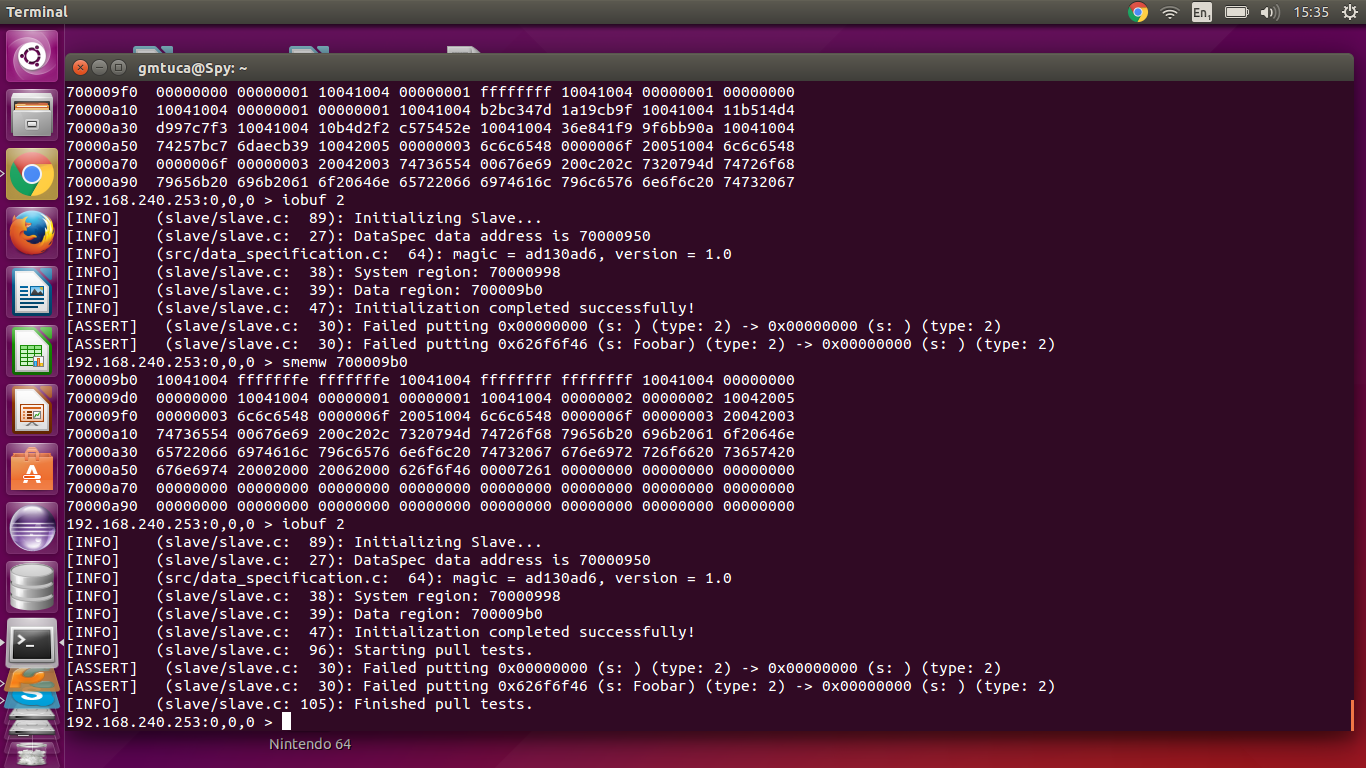
\includegraphics[width=1.3\linewidth, natwidth=1366, natheight=768]{images/debugging.png}
  \captionof{figure}{Debugging}
  \label{fig:debugging}
  \centering
  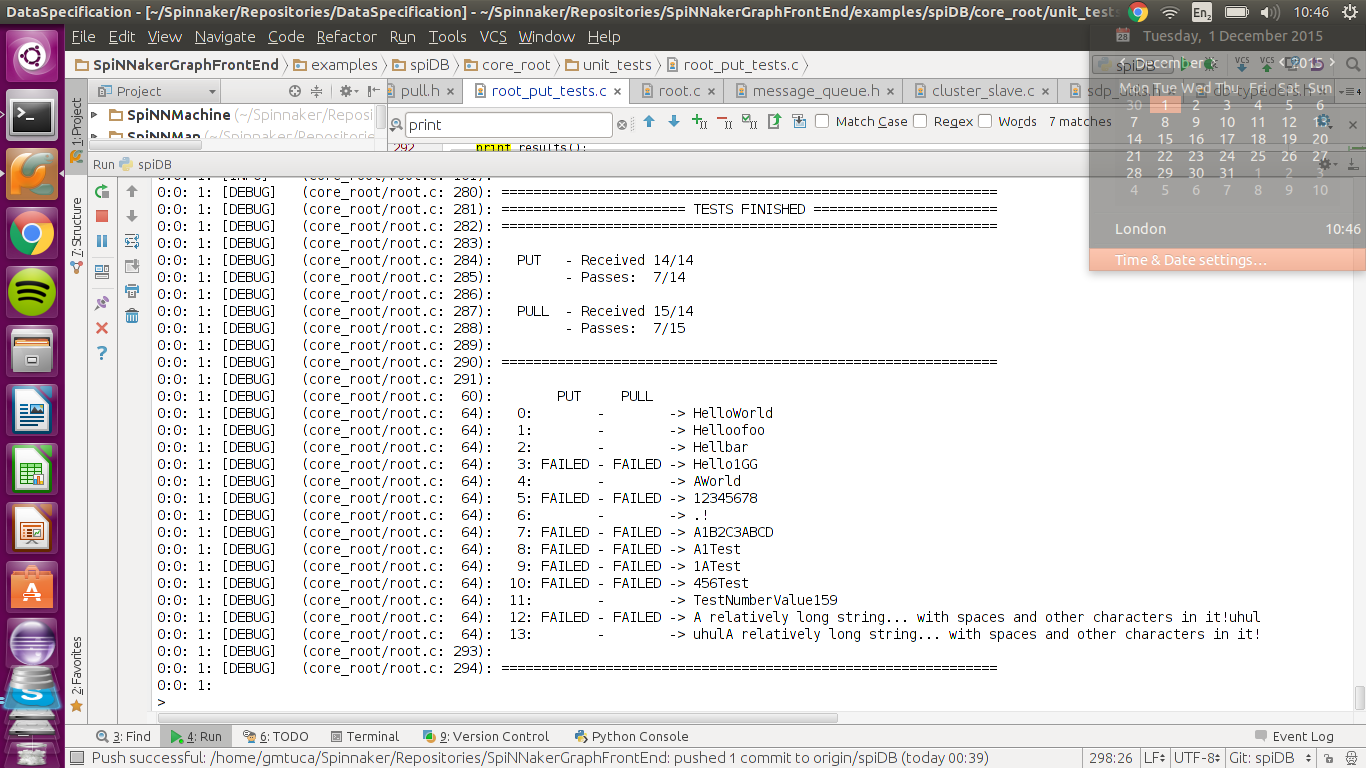
\includegraphics[width=1.3\linewidth, natwidth=1366, natheight=768]{images/testing.png}
  \captionof{figure}{Testing}
  \label{fig:testing}
\end{figure}


\section{Bugs}
I have been one of the few users of a large amount of the SpiNNaker API, currently under contruction. This means some of it has not been fully tested, resulting in strange behaviour at times, making debugging of my own application difficult.

blah blah test usability
particularly

Although not being directly part of the project, 

MENTORING

\begin{itemize}
\item \textbf{Duplicate packets:} when multiple distinct SDP packets were sent from different sources to the same destination, strangely the receiving core would read the same packet duplicated a number of times. This behaviour was unexpected, so upon extensive testing and collaboration from the team, I was able to point the issue to a running processor binary named \textit{reinjector} and resolve the issue. 

\item \textbf{Data Specification Error:} when uploading binaries to the board, sometimes cores would crash with the SWERR state. After giving the team detailed feedback on the issue, this was found to be caused by the SpiNNaker Data Specification framework, which handles allocation of data in shared RAM.

\item algorithms

\end{itemize}

From planning, design, testing, development, code review, etc. presentation of results to members of the Spinnaker team

It outlines also my approach and design choices with their advantages/disadvantages with the hardware and specification. (eg. no acknowledgements)
Approval from members of the SpiNNaker team.

Strengths and weaknesses (limitations) of spinnaker
...
Thomas, etc.
tutoring! kind of did it really

...upload different programs to run on each core.
Thus each chip contains the following instances: 

Bizantine protocol
